\documentclass[11pt]{article}

% robustness: Times for text and math, core packages only
\usepackage[T1]{fontenc}
\usepackage[utf8]{inputenc}
\usepackage[margin=1.1in]{geometry}
\usepackage{mathptmx}              % Times for text + math
\usepackage{amsmath,amssymb}
\usepackage{graphicx}
\usepackage{booktabs}
\usepackage{caption}
\usepackage{float}
\usepackage{enumitem}
\usepackage[hidelinks]{hyperref}
\usepackage{microtype}             % tighter, less cramped justification

\hypersetup{
  bookmarksnumbered=true,
  bookmarksopen=true,
  bookmarksopenlevel=1,
  pdftitle={Test-Time Training on a Budget: ARC-AGI-2 on a Single Consumer GPU},
  pdfauthor={ARC Prize 2026 Paper Track entry}
}

\graphicspath{{./}}
\captionsetup{font=small,labelfont=bf}
\linespread{1.1}                   % more leading, less cramped
\setlength{\parskip}{0.55em}
\setlength{\parindent}{0pt}
\DeclareMathOperator*{\select}{select}   % top-2 vote selection operator

\title{\textbf{Test-Time Training on a Budget:\\[2pt] ARC-AGI-2 on a Single Consumer GPU}}
\author{ARC Prize 2026 Paper Track entry}
\date{}

\begin{document}

\begin{titlepage}
\centering
\vspace*{0.10\textheight}
{\Huge\bfseries Test-Time Training on a Budget\par}
\vspace{0.7em}
{\LARGE\bfseries ARC-AGI-2 on a Single Consumer GPU\par}
\vspace{1.1em}
{\large Running the 2025 ARC Prize winning recipe, per-task test-time training\\[3pt]
with augment-infer-reverse-vote selection, on one 16~GB card\par}
\vspace{0.045\textheight}
\rule{0.55\linewidth}{0.4pt}\par
\vspace{0.05\textheight}
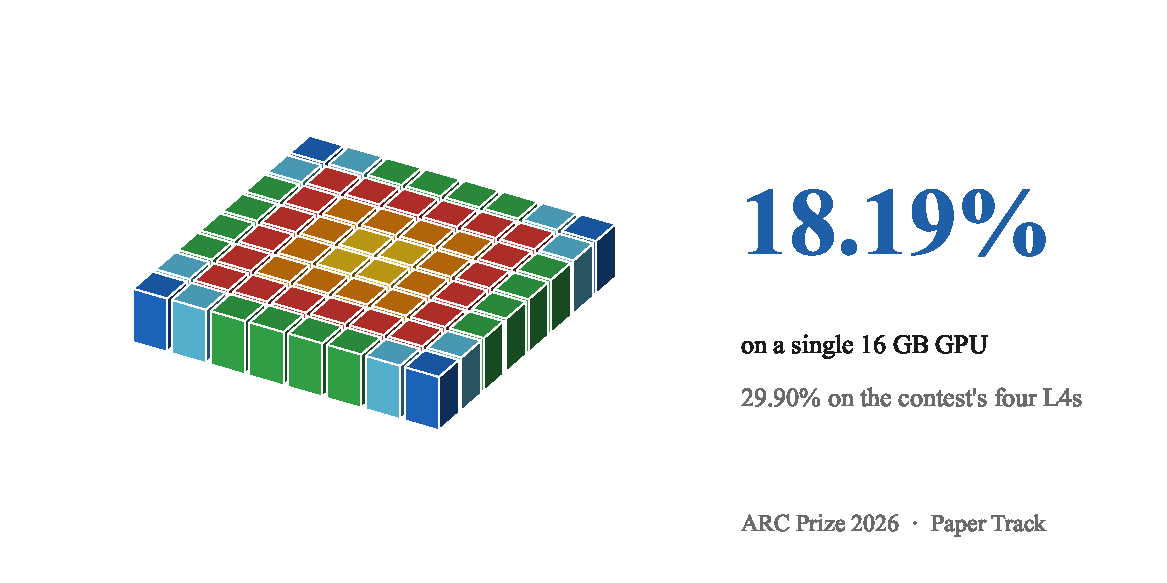
\includegraphics[width=0.94\linewidth]{cover_hero}\par
\vspace{\fill}
{\large ARC Prize 2026 Paper Track entry\par}
\vspace{0.5em}
{\normalsize Open source under MIT-0\par}
\vspace*{0.06\textheight}
\end{titlepage}

\begin{abstract}
The strongest published results on ARC-AGI-2 come from multi-GPU clusters. We ask how far the 2025
winning recipe, a small grid language model with per-task test-time training (TTT) and
Augment-Infer-Reverse-Vote (AIRV) selection, goes on a single 16~GB consumer GPU, and where it walls
out. Building on the released NVARC Qwen3-4B grid model, we report a reproducible offline system with
a \textbf{12.79\%} no-TTT baseline on the 120-task public evaluation set, and 6.53\% on the hidden main-track
leaderboard. We find that the binding
constraint is generation throughput, not model quality or memory, and that the single largest lever
is the inference engine, which buys a $13\times$ decode speedup. We then show how to run per-task TTT
on this hardware by serving each task's adapter on the fast engine, and report a measured lift: naive
TTT ties the no-TTT baseline because the per-task adapter overfits, while a regularized, scale-tuned
configuration raises accuracy from 12.8\% to \textbf{17.6\%} on the 84 trainable tasks, lifting the
full evaluation to a blended \textbf{16.28\%}. The contribution is an honest accounting of what the
recipe costs and where the effort should go when you cannot rent a cluster. All code, the conversion
recipe, and a development log of every measurement are open source under MIT-0.
\end{abstract}

{\small\tableofcontents}
\medskip

\noindent\textbf{Reader's guide.} Section~\ref{sec:intro} motivates efficient ARC and states the
contributions. Section~\ref{sec:related} places the work against the 2025 winning systems.
Section~\ref{sec:method} is the method: the model and prompt format (\ref{sec:model}), the engine
bottleneck and its fix (\ref{sec:engine}), the AIRV selection rule (\ref{sec:airv}), and the per-task
TTT bridge (\ref{sec:ttt}). Section~\ref{sec:results} reports the numbers; Section~\ref{sec:disc}
draws the lessons. Readers who want to reproduce the system should go straight to
Appendix~\ref{app:repro}; the per-scale tables and significance detail are in
Appendix~\ref{app:results}; the honest list of dead ends is Appendix~\ref{app:log}; the exact prompt
and 16-token vocabulary are in Appendix~\ref{app:format}; data licensing and BibTeX are in
Appendix~\ref{app:prov}.

\section{Introduction}
\label{sec:intro}

\subsection{Efficient abstraction is the point}
ARC-AGI-2~\cite{chollet,arcagi2} is a benchmark of abstraction and reasoning: each task gives a few
input/output grid pairs that demonstrate a transformation, and the solver must apply that
transformation to a held-out input. The tasks are designed to be easy for humans and hard for
machines, and the competition is run \emph{offline}, which rules out frontier API models and forces
every entrant to ship a self-contained system. The 2025 ARC Prize was won by NVARC at 24.0\% on
ARC-AGI-2 using a 4B grid model with per-task TTT~\cite{arc2025,nvarc}; the recipe reproduced across
the top teams is the same: fine-tune a small model on augmented grid data, train a fresh low-rank
adapter on each test task, then sample many augmented candidates and vote.

The recipe is effective but expensive: the public reports were produced on clusters of H100 or GH200
GPUs. Most researchers do not have that hardware, and the ARC Prize's stated mission is
\emph{efficient} skill acquisition, not skill bought with compute. We therefore characterize the
recipe under a constraint we think is widely shared: a single RTX~5070~Ti with 16~GB, on the
Blackwell architecture, running native Windows. The aim is not to top the leaderboard, which is
unrealistic on one card, but to build a working, reproducible system, measure honest numbers, and map
where one card stops being enough. Figure~\ref{fig:solve} shows a representative task our system
solves end to end.

\begin{figure}[H]
\centering
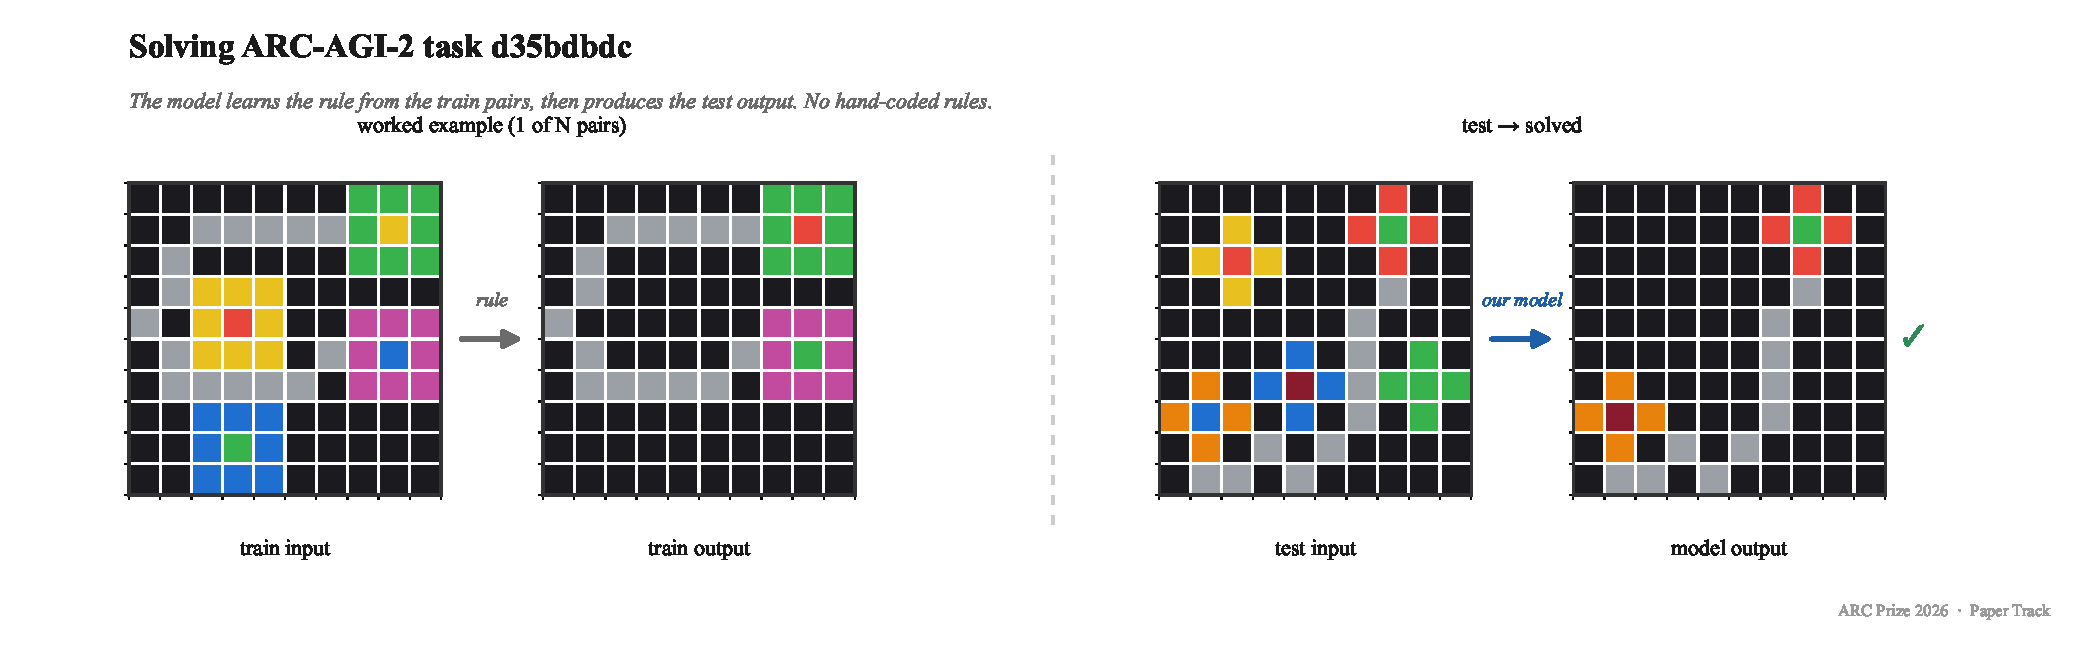
\includegraphics[width=0.92\linewidth]{fig_solve}
\caption{A real ARC-AGI-2 evaluation task solved by the no-TTT pipeline, shown as colour grids: the
few-shot train pairs establish the rule, and the model produces the held-out test output exactly.
Grids are rendered with the model's own 16-colour serialization (Appendix~\ref{app:format}).}
\label{fig:solve}
\end{figure}

\subsection{Contributions}
\begin{enumerate}[leftmargin=1.4em,itemsep=2pt]
\item A reproducible offline ARC-AGI-2 system for the custom-vocabulary NVARC model on a single
16~GB card, with a clean \textbf{12.79\%} no-TTT baseline (Section~\ref{sec:results},
Appendix~\ref{app:repro}).
\item The finding that, on this hardware class, the inference \emph{engine} dominates every other
knob: moving decode off the Hugging Face eager path onto llama.cpp is worth a $13\times$ speedup
(Section~\ref{sec:engine}).
\item A practical bridge that makes per-task TTT runnable on one card by hot-swapping GGUF adapters
on the fast engine, and a measured, regularization-dependent lift to a \textbf{16.28\%} blend
(Section~\ref{sec:ttt}, \ref{sec:ttt-results}).
\item An ``accuracy per GPU-hour'' accounting that names the three walls a compute-poor practitioner
hits first: the decode ceiling, the VRAM limit on large-grid TTT, and adapter overfitting
(Section~\ref{sec:disc}).
\item A complete open-source release: the conversion patches, the pipeline, the TTT harness, and a
development log of every measurement and dead end behind these numbers (Appendix~\ref{app:log}).
\end{enumerate}

\section{Related Work}
\label{sec:related}

\textbf{ARC and the measure of intelligence.} ARC was introduced to measure skill-acquisition
efficiency rather than skill itself~\cite{chollet}; ARC-AGI-2~\cite{arcagi2} raises compositional
difficulty while keeping tasks human-solvable, widening the human/machine gap that frontier models
had begun to close on ARC-AGI-1.

\textbf{Test-time training.} The dominant 2025 approach fits a small per-task adapter at inference,
trading test-time compute for generalization. The ARC Prize 2025 technical report~\cite{arc2025}
identifies this, together with heavy synthetic pre-training and disciplined engineering, as the core
of the winning NVARC solution~\cite{nvarc}, whose released model we build on directly. We hold this
recipe fixed and ask what survives a single consumer GPU.

\textbf{Augmentation and voting.} Predicting under the eight dihedral symmetries of the grid,
inverting each prediction back to the original frame, and voting is a standard self-consistency
device for ARC; it is cheap, training-free, and provides a usable confidence signal
(Section~\ref{sec:airv}).

\textbf{Synthetic data.} Procedural generators such as RE-ARC~\cite{rearc} and LLM-mutated corpora
supply the augmented grid data these models are trained on. We use RE-ARC only in an in-progress
base-model probe (Section~\ref{sec:limits}), not in the results below.

\textbf{Efficient and on-device inference.} Our engineering contribution, getting a custom-vocabulary
grid transformer to decode near the memory-bandwidth roofline on a consumer card and then serving
per-task adapters on it, sits in the practical lineage of quantized GGUF inference. The novelty is
not the engine but the demonstration that the full TTT recipe, adapter serving included, fits one
16~GB card, and a measurement of exactly where it stops.

\section{System and Method}
\label{sec:method}

\subsection{Model and prompting}
\label{sec:model}
We use the NVARC \texttt{qwen3\_4b\_grids15\_sft139} model, a Qwen3-4B~\cite{qwen3} with a 16-token
vocabulary: the ten grid colours as digits, a newline, two role markers, and three specials
(Appendix~\ref{app:format}). A grid is serialized one token per cell, and a colour value equals its
token id. Because the role and special tokens cannot be produced by tokenizing text, we assemble
every prompt at the token-id level as a ChatML few-shot sequence; getting this byte-exact is the
single most important correctness condition, since a one-token drift between training and inference
silently destroys accuracy.

\subsection{The engine is the bottleneck}
\label{sec:engine}
Our most consequential finding concerns throughput. Decoding a 4B model is memory-bound: each token
streams the full weight matrix from VRAM, so for a weight footprint $M$ on a card of bandwidth $B$
the decode rate is bounded by a first-order roofline
\begin{equation}
r_{\max} \;=\; \frac{B}{M}.
\label{eq:roofline}
\end{equation}
With $B=896$~GB/s, Eq.~\eqref{eq:roofline} gives $132$ tok/s in bf16 ($M=6.77$~GB), $249$ in Q8\_0
($M=3.6$~GB), and $444$ in Q4\_K\_M ($M=2.02$~GB). The standard Hugging Face eager path prefills
healthily ($\approx 3{,}400$ tok/s) but \emph{decodes} at only $\approx 13$ tok/s, about a tenth of
the bf16 roof, because of per-token framework overhead with no CUDA graphs. The usual remedy,
compiling the decode step, is unavailable on this platform: \texttt{torch.compile} needs Triton, and
Triton has no native-Windows backend (Appendix~\ref{app:log}).

The fix is to change engines. We convert the model to GGUF and serve it with llama.cpp. The custom
vocabulary needs two small, documented converter patches (Appendix~\ref{app:repro}): the unknown
tokenizer hash is mapped to the \texttt{qwen2} pre-tokenizer it actually uses, and two throwaway
byte-pair merges are added to satisfy a loader that requires a non-empty merge list (they never fire
on grid text). The prebuilt CUDA~12.4 binary runs on the Blackwell card through PTX just-in-time
compilation. Measured decode rises to $102$ tok/s in bf16, $170$ in Q8\_0, and $244$ in Q4\_K\_M
(Figure~\ref{fig:roofline}), a $13\times$ speedup over eager at Q8\_0, which we adopt: it is
near-lossless (14 of 15 training tasks reproduced exactly under greedy decoding) and has a 3.6~GB
footprint. One stability note: the server's default prompt cache reserves $\approx 680$~MiB per
unique prompt; since every ARC prompt is unique it yields no reuse and destabilizes sustained
generation, so we disable it and run a single supervised stream.

\begin{figure}[H]
\centering
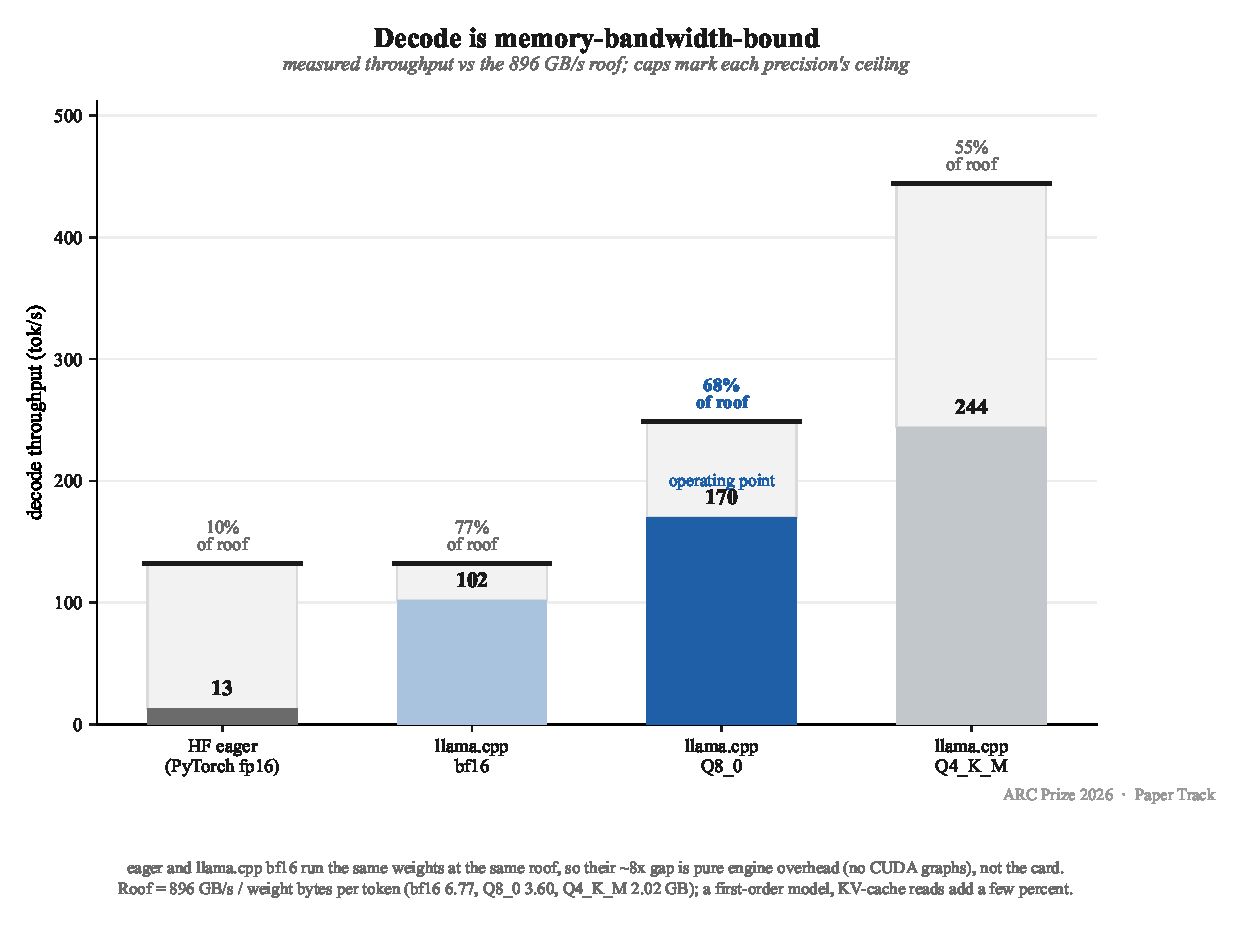
\includegraphics[width=0.84\linewidth]{fig_roofline}
\caption{Decode throughput versus the memory-bandwidth roofline of Eq.~\eqref{eq:roofline} (the
ceiling is a first-order model, bytes/token $\approx$ weight bytes). Bars are \emph{measured} tok/s;
the shaded gap to each cap is framework overhead, not the card. The eager path fills only $\approx
10\%$ of its roof; moving decode to llama.cpp at Q8\_0 recovers the $13\times$.}
\label{fig:roofline}
\end{figure}

\subsection{AIRV: augment, infer, reverse, vote}
\label{sec:airv}
Let $f$ be the served model and $\mathcal{G}$ the eight dihedral (D4) symmetries of the grid. For a
test input $x$ we generate one prediction per symmetry, invert it back to the original frame, and
vote. Writing $n_c$ for a candidate's vote count and $\bar{\ell}_c$ for its mean sequence log-prob,
\begin{equation}
c_g \;=\; g^{-1}\!\big(f(g(x))\big),\qquad
\hat{Y} \;=\; \select_{c}\ \big(\,n_c,\ \bar{\ell}_c\,\big),\qquad
n_c=\big|\{g\in\mathcal{G}: c_g=c\}\big|,\quad
\bar{\ell}_c=\tfrac{1}{n_c}\!\!\sum_{g:\,c_g=c}\!\!\log p(c_g),
\label{eq:airv}
\end{equation}
where $\select$ returns the two distinct candidates with the highest vote count, ties broken by mean
log-prob, and emits them as the two attempts the metric allows. The vote count is itself a usable
confidence signal: agreement across symmetries predicts correctness (Figure~\ref{fig:votes}). The
whole offline system (the trainer, the converter, and the server, which never share VRAM) is sketched
in Figure~\ref{fig:pipeline}.

\begin{figure}[H]
\centering
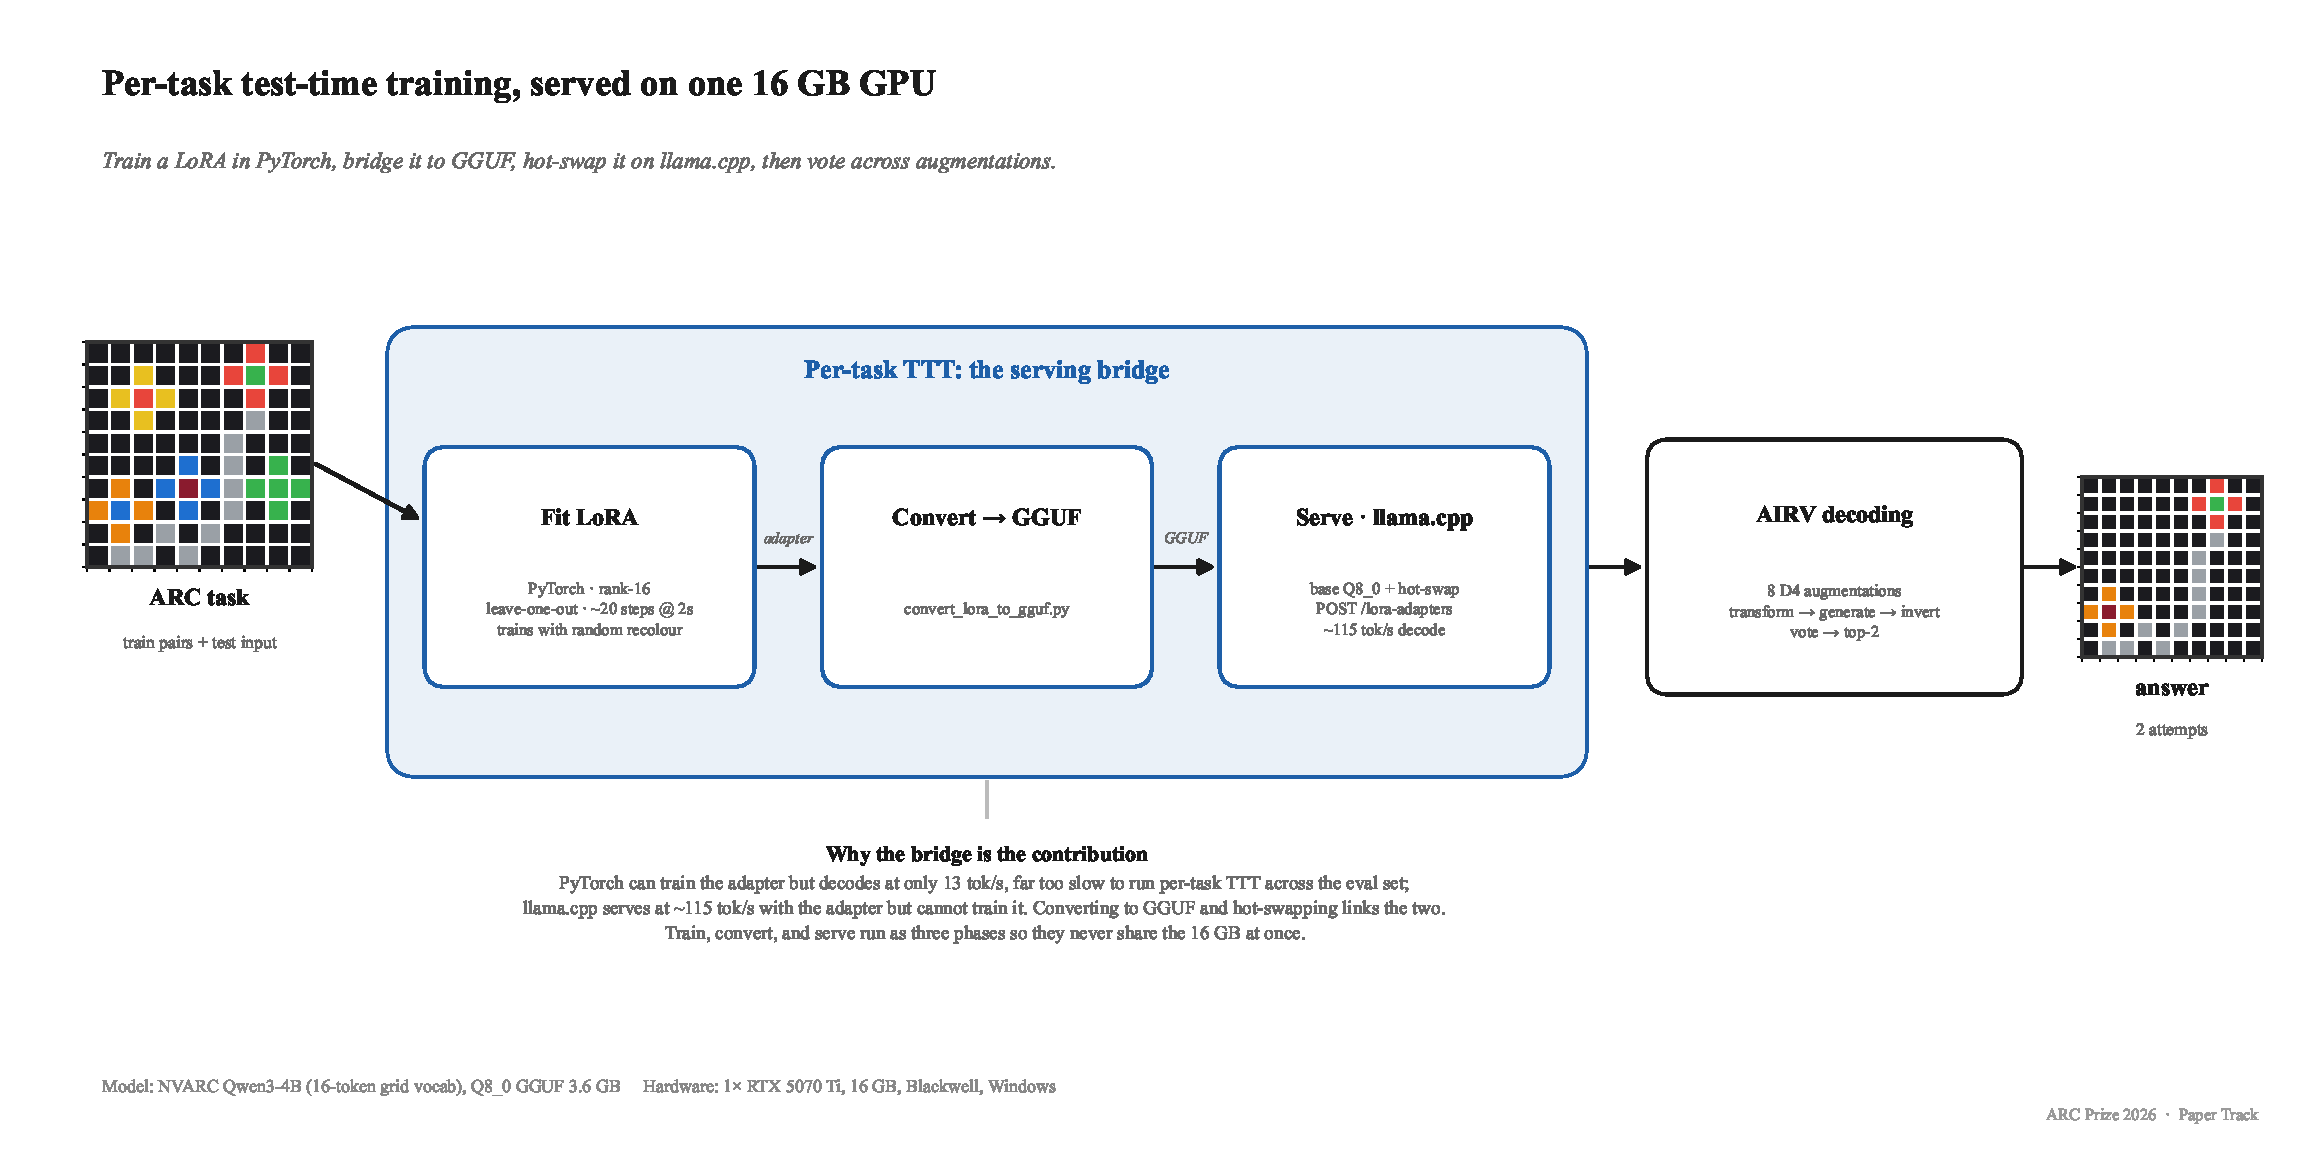
\includegraphics[width=\linewidth]{fig_pipeline}
\caption{The offline system. The PyTorch trainer and the llama.cpp server never share VRAM; per-task
adapters cross the bridge as GGUF and are hot-swapped on the fast engine per request.}
\label{fig:pipeline}
\end{figure}

\subsection{Per-task test-time training}
\label{sec:ttt}
For TTT we fit a per-task LoRA adapter $\Delta W = s\,BA$ of rank $r$ and scale $s$ on the task's own
train pairs $T$, with a leave-one-out target and the loss masked to the answer tokens:
\begin{equation}
\mathcal{L}(\theta) \;=\; -\!\!\sum_{(u,v)\in T}\ \sum_{t}
\log p_{\theta}\big(v_t \mid v_{<t},\, \mathrm{ctx}_{\,T\setminus\{(u,v)\}},\, u\big),
\label{eq:ttt}
\end{equation}
drawing a fresh random augmentation each step. Capping the few-shot context to $\approx 1{,}600$
tokens drops a training step from $\approx 13$~s to $\approx 2$~s, so training is no longer the
expensive part.

The harder problem is \emph{serving} the trained adapter. TTT must run in PyTorch, where decoding is
the slow 13 tok/s and intermittently becomes quadratic after a step; the fast engine does not train.
We bridge them (Figure~\ref{fig:pipeline}): train in PyTorch, save each adapter, convert it to a GGUF
adapter, and hot-swap it on llama.cpp through its \texttt{/lora-adapters} endpoint, where decode
holds $\approx 115$ tok/s with no stalls. We run three phases (train all, convert all from a clean
process, then serve and generate all) so the two frameworks never share VRAM
(Figure~\ref{fig:phases}). Large-grid tasks remain too VRAM-bound to train and are excluded by their
largest-train-pair token length (Figure~\ref{fig:vram}).

\begin{figure}[H]
\centering
\begin{minipage}{0.49\linewidth}\centering
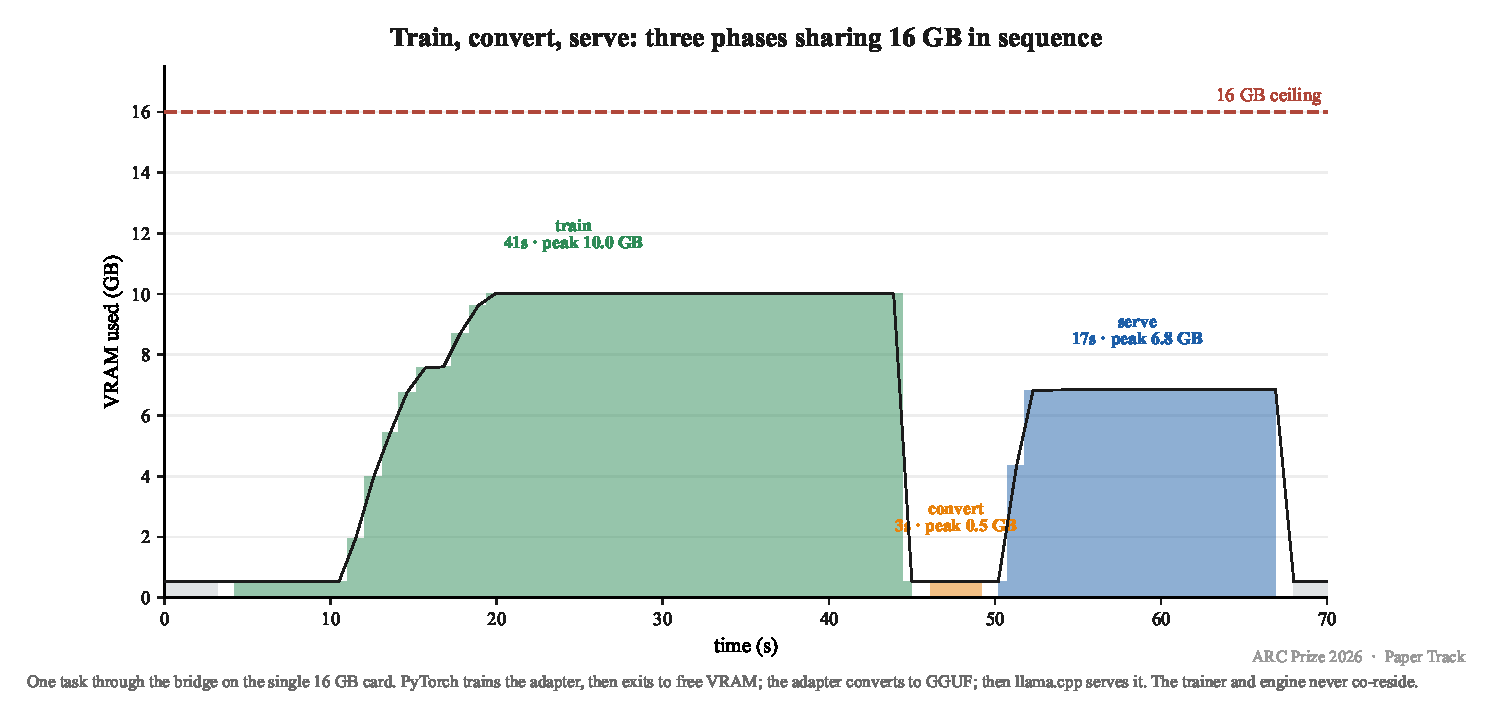
\includegraphics[width=\linewidth]{fig_phases}
\end{minipage}\hfill
\begin{minipage}{0.49\linewidth}\centering
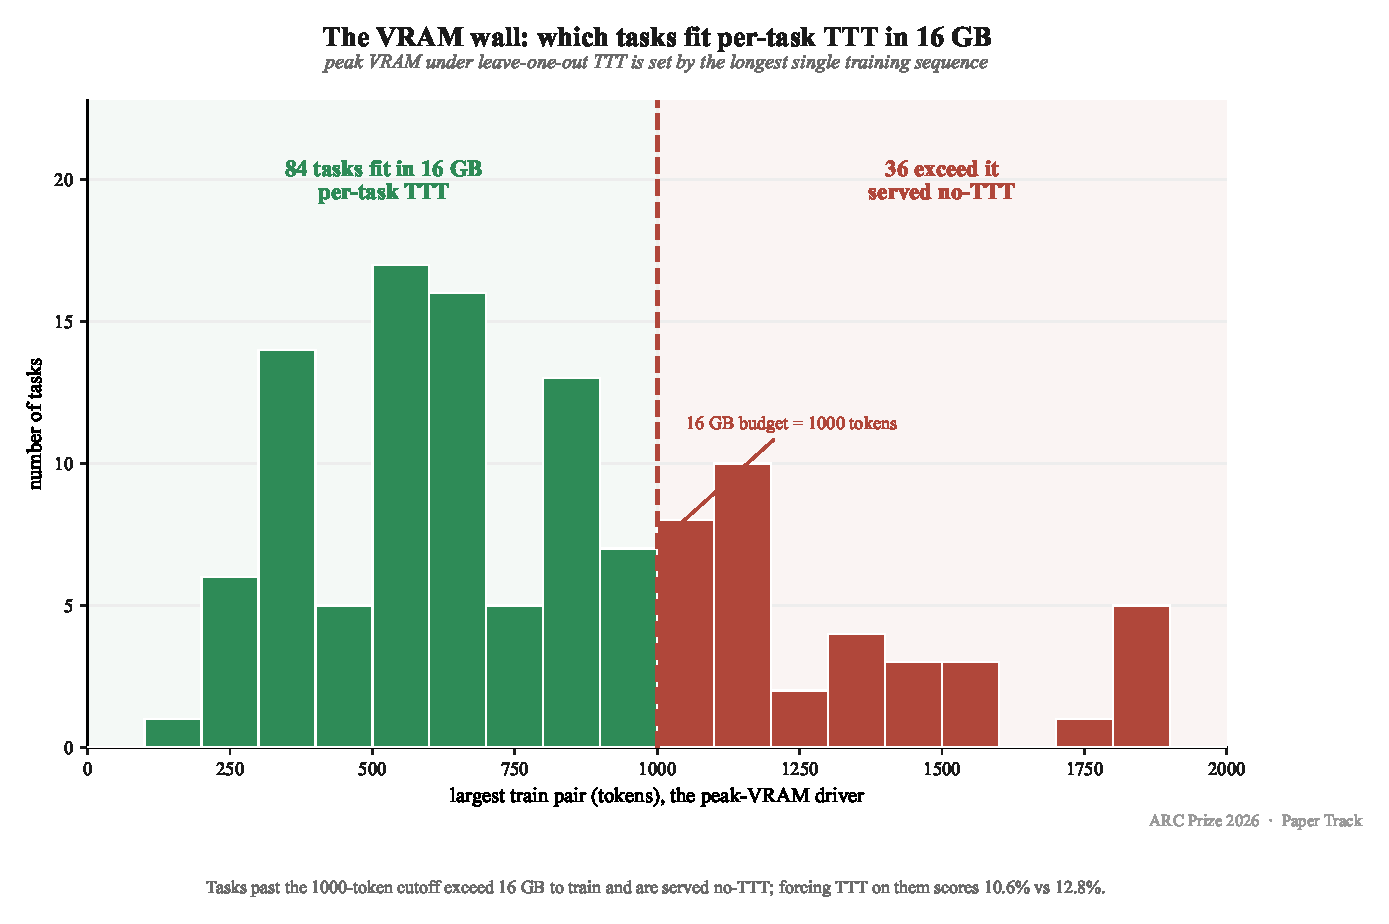
\includegraphics[width=\linewidth]{fig_vram_wall}
\end{minipage}
\caption{Left: the three-phase schedule keeps PyTorch and llama.cpp from sharing the 16~GB at once
(VRAM trace sampled live; peaks measured). Right: the VRAM wall, with each task placed by grid size
and context length; tasks above the operational cutoff are excluded from TTT (the cutoff metric is
the largest train pair, and any VRAM surface shown is a calibrated model).}
\label{fig:phases}
\label{fig:vram}
\end{figure}

\section{Results}
\label{sec:results}

\subsection{No-TTT baseline}
The AIRV pipeline without TTT scores \textbf{12.79\%} (22 of 172 test outputs) on the 120-task public
evaluation set, a clean single-stream run completing in $\approx 78$ minutes. Submitted to the
ARC-AGI-2 main-track leaderboard, the same pipeline scores \textbf{6.53\%} on the hidden 240-task
test set (semi-private plus private), a roughly twofold drop from the public eval that we attribute
to the hidden set's greater difficulty, and possibly to per-task failures in the scored rerun
(Section~\ref{sec:limits}). For reference the 2025 winner reached 24.0\% with TTT~\cite{arc2025}.

\subsection{The engine speedup}
The $13\times$ decode improvement from changing engines (Section~\ref{sec:engine},
Figure~\ref{fig:roofline}) is the single most important result for this hardware class. It turned an
overnight, frequently-failing process into a sub-90-minute evaluation. On one consumer GPU, the
inference engine dominated every other knob we touched (Figure~\ref{fig:results}).

\begin{figure}[H]
\centering
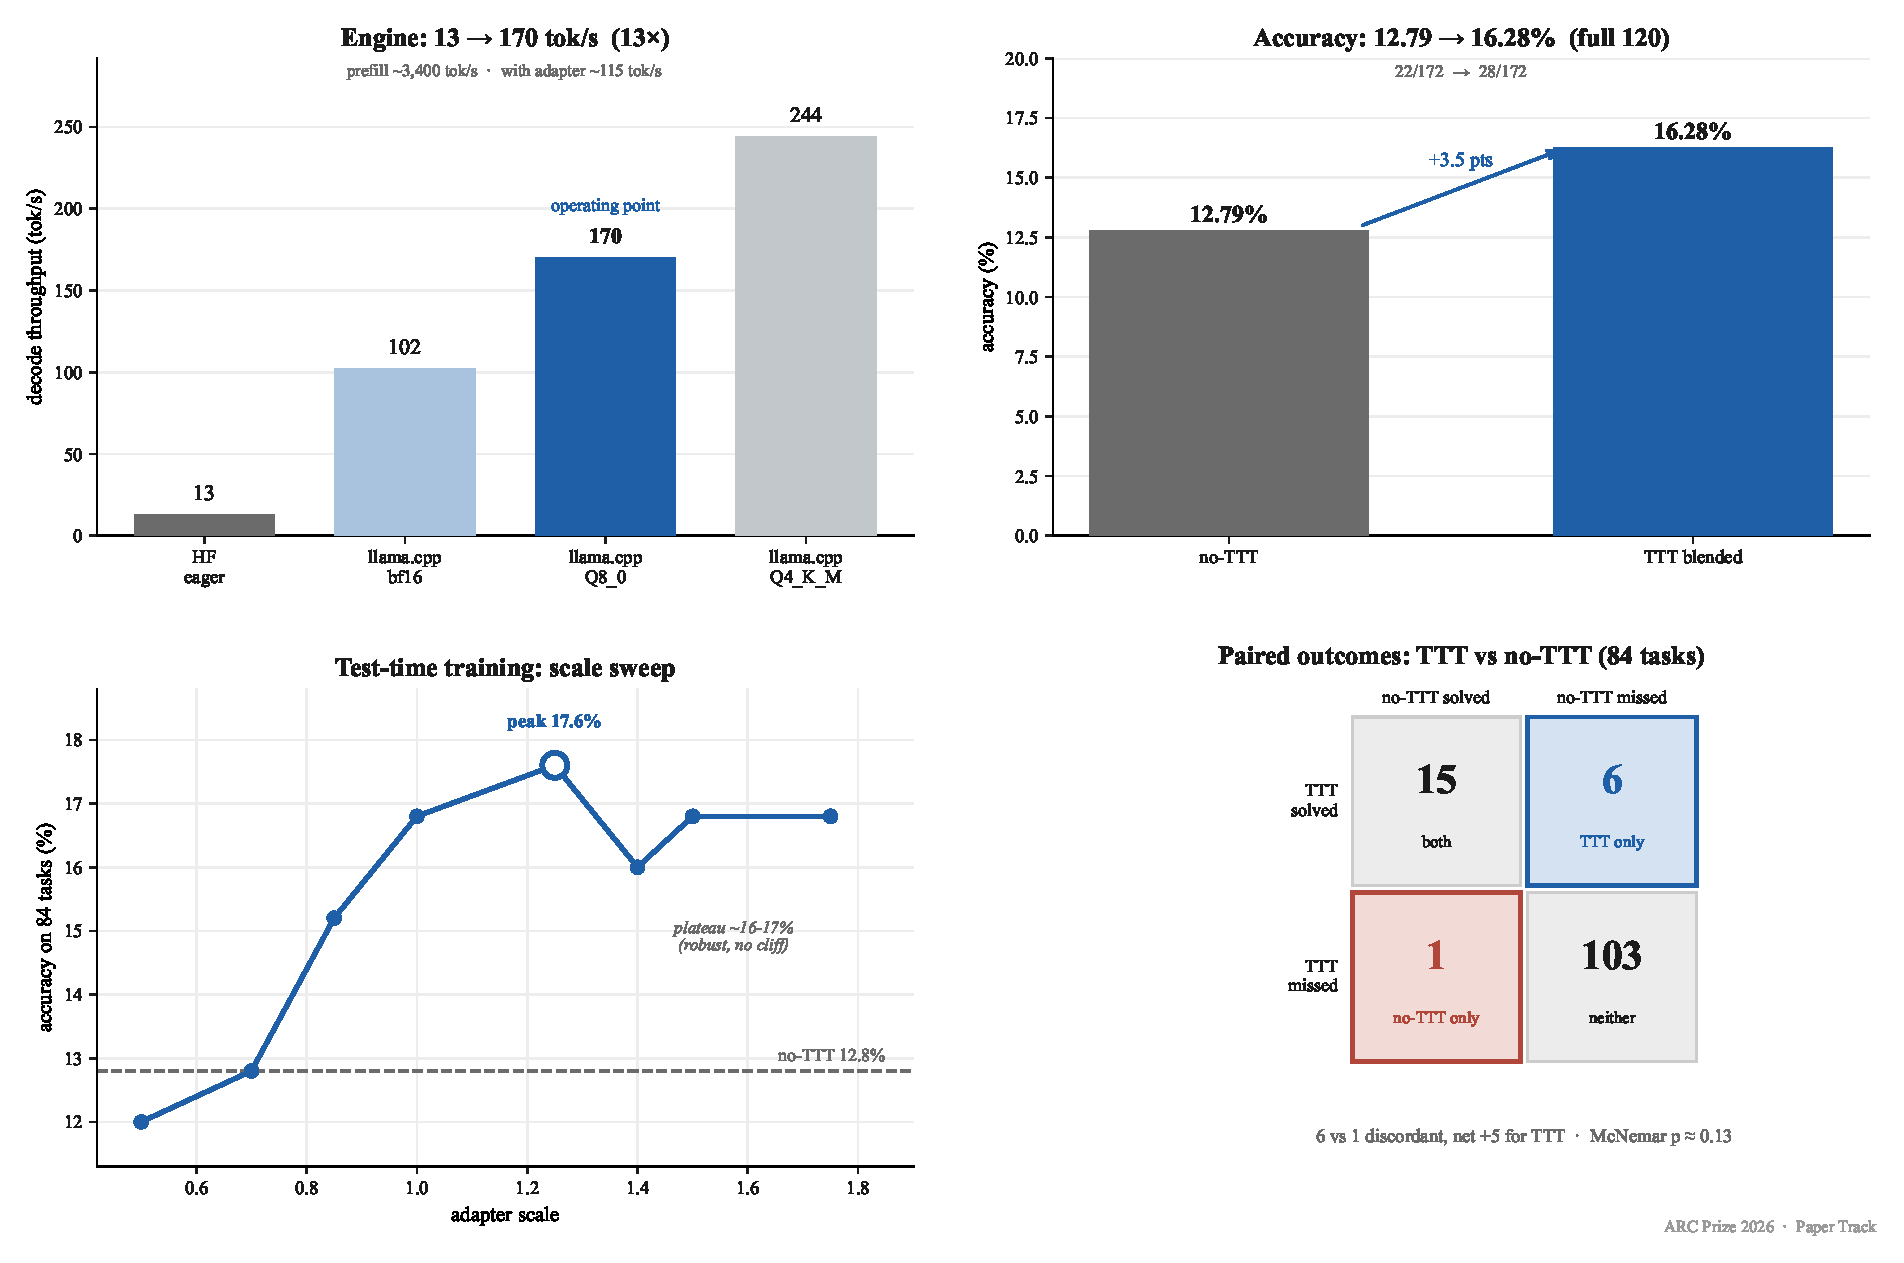
\includegraphics[width=\linewidth]{fig_results}
\caption{Engine choice, accuracy, and the adapter-scale curve. Accuracy peaks at scale $1.25$ on the
84 trainable tasks, then declines, a real optimum rather than a monotone gain. All values are
measured.}
\label{fig:results}
\end{figure}

\subsection{Test-time training}
\label{sec:ttt-results}
With generation fixed, we first swept the adapter configuration on 15 small-context tasks, scoring
each against no-TTT on the same tasks (Table~\ref{tab:sweep}). The standard configuration overfits
(its training loss reaches $0.000$) and ties the baseline; the regularized configuration recovers a
one-task lift; an over-aggressive reduction undertrains and ties again, coherent with an overfit
diagnosis, though one task on 15 is only a hint.

\begin{table}[H]
\centering
\caption{Adapter-configuration sweep on 15 small-context tasks (23 test outputs).}
\label{tab:sweep}
\begin{tabular}{lcc}
\toprule
configuration & TTT & no-TTT \\
\midrule
40 steps, rank 32, no dropout      & 3/23 & 3/23 \\
20 steps, rank 16, dropout 0.1     & \textbf{4/23} & 3/23 \\
8 steps, rank 8, dropout 0.05      & 3/23 & 3/23 \\
\bottomrule
\end{tabular}
\end{table}

We then validated the regularized configuration at scale, on the 84 evaluation tasks small enough to
train on a 16~GB card, against no-TTT on the same tasks (Table~\ref{tab:scale}). The lift holds and
strengthens: $+5$ test outputs, a four-point gain ($\approx 31\%$ relative). The paired breakdown is
clean: of the tasks the two methods disagree on, TTT is right on six that no-TTT misses and wrong on
only one. With seven disagreements this is not individually significant (exact McNemar
$p\approx0.13$, Appendix~\ref{app:results}), but three measurements now agree in direction (sweep
$+1$, scale $+5$, six-to-one discordant), and no-TTT scores 12.8\% here against its 12.79\% full
baseline, so the subset is representative.

\begin{table}[H]
\centering
\caption{Regularized TTT vs.\ no-TTT on the 84 trainable tasks (125 test outputs), scale $1.0$.}
\label{tab:scale}
\begin{tabular}{lcc}
\toprule
method & correct & accuracy \\
\midrule
regularized TTT & \textbf{21/125} & \textbf{16.8\%} \\
no-TTT          & 16/125 & 12.8\% \\
\bottomrule
\end{tabular}
\end{table}

\subsection{Ablations: scale, colour, and the big-grid wall}
Three further levers, each measured on the 84 trainable tasks (full per-scale numbers in
Appendix~\ref{app:results}). The adapter \emph{scale} matters: accuracy peaks at 17.6\% at scale
$1.25$, then declines (Figures~\ref{fig:results},~\ref{fig:flip}). Colour permutation lifts the
no-TTT baseline to 14.4\% but does \emph{not} stack with the already colour-robust adapter. Forcing
TTT onto the big-grid tasks does not help; the VRAM exclusion is a genuine ceiling, not a missed
opportunity. The best blend, TTT at scale $1.25$ where trainable and no-TTT elsewhere, reaches
\textbf{16.28\%} on the full 120-task evaluation, up from 12.79\%. The honest summary: naive per-task
TTT \emph{ties} a strong no-TTT AIRV baseline, while a regularized, scale-tuned TTT \emph{beats} it by
a consistent if modest margin.

\begin{figure}[H]
\centering
\begin{minipage}{0.56\linewidth}\centering
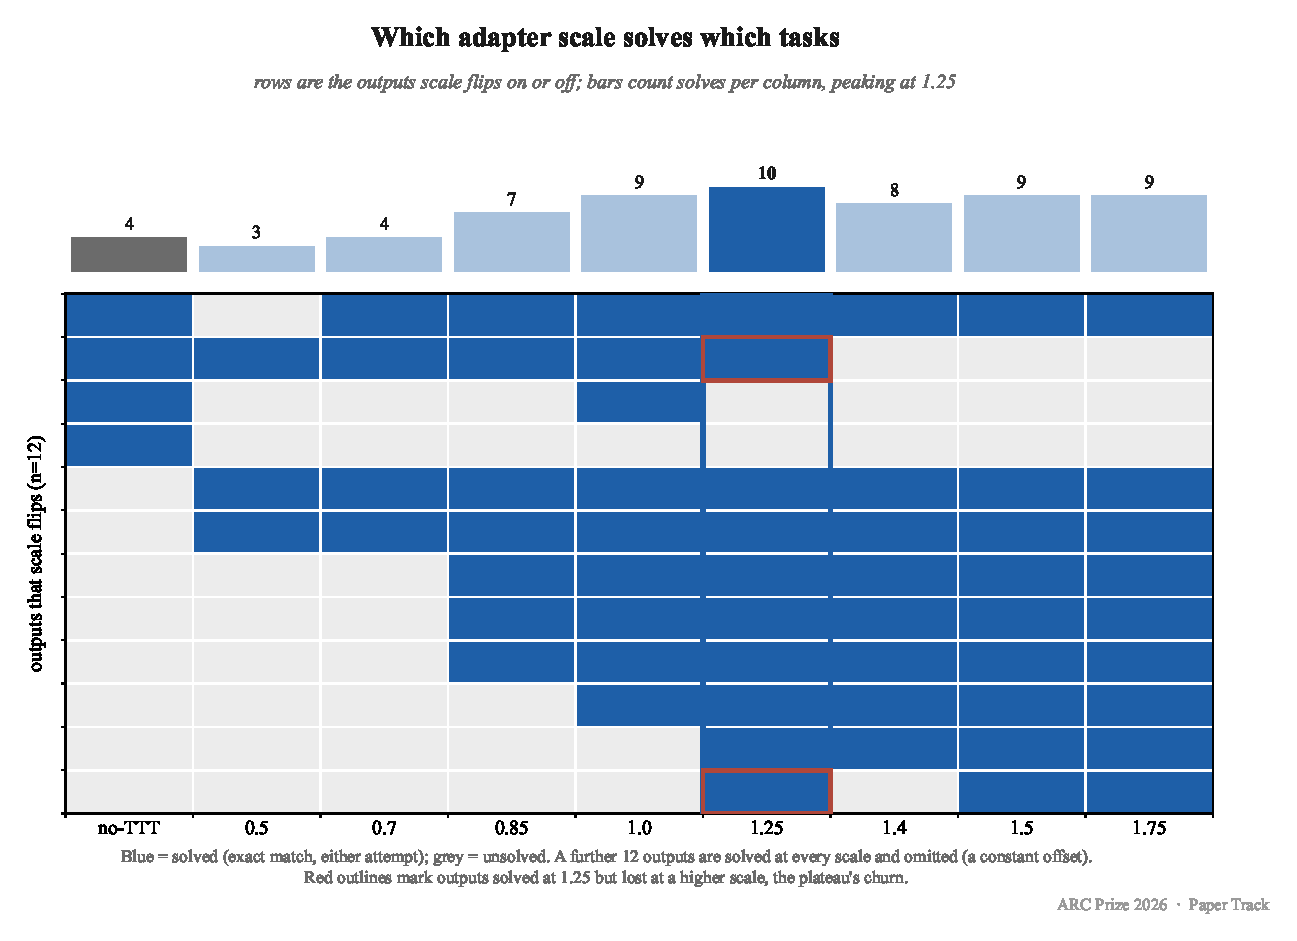
\includegraphics[width=\linewidth]{fig_scale_flip}
\end{minipage}\hfill
\begin{minipage}{0.42\linewidth}\centering
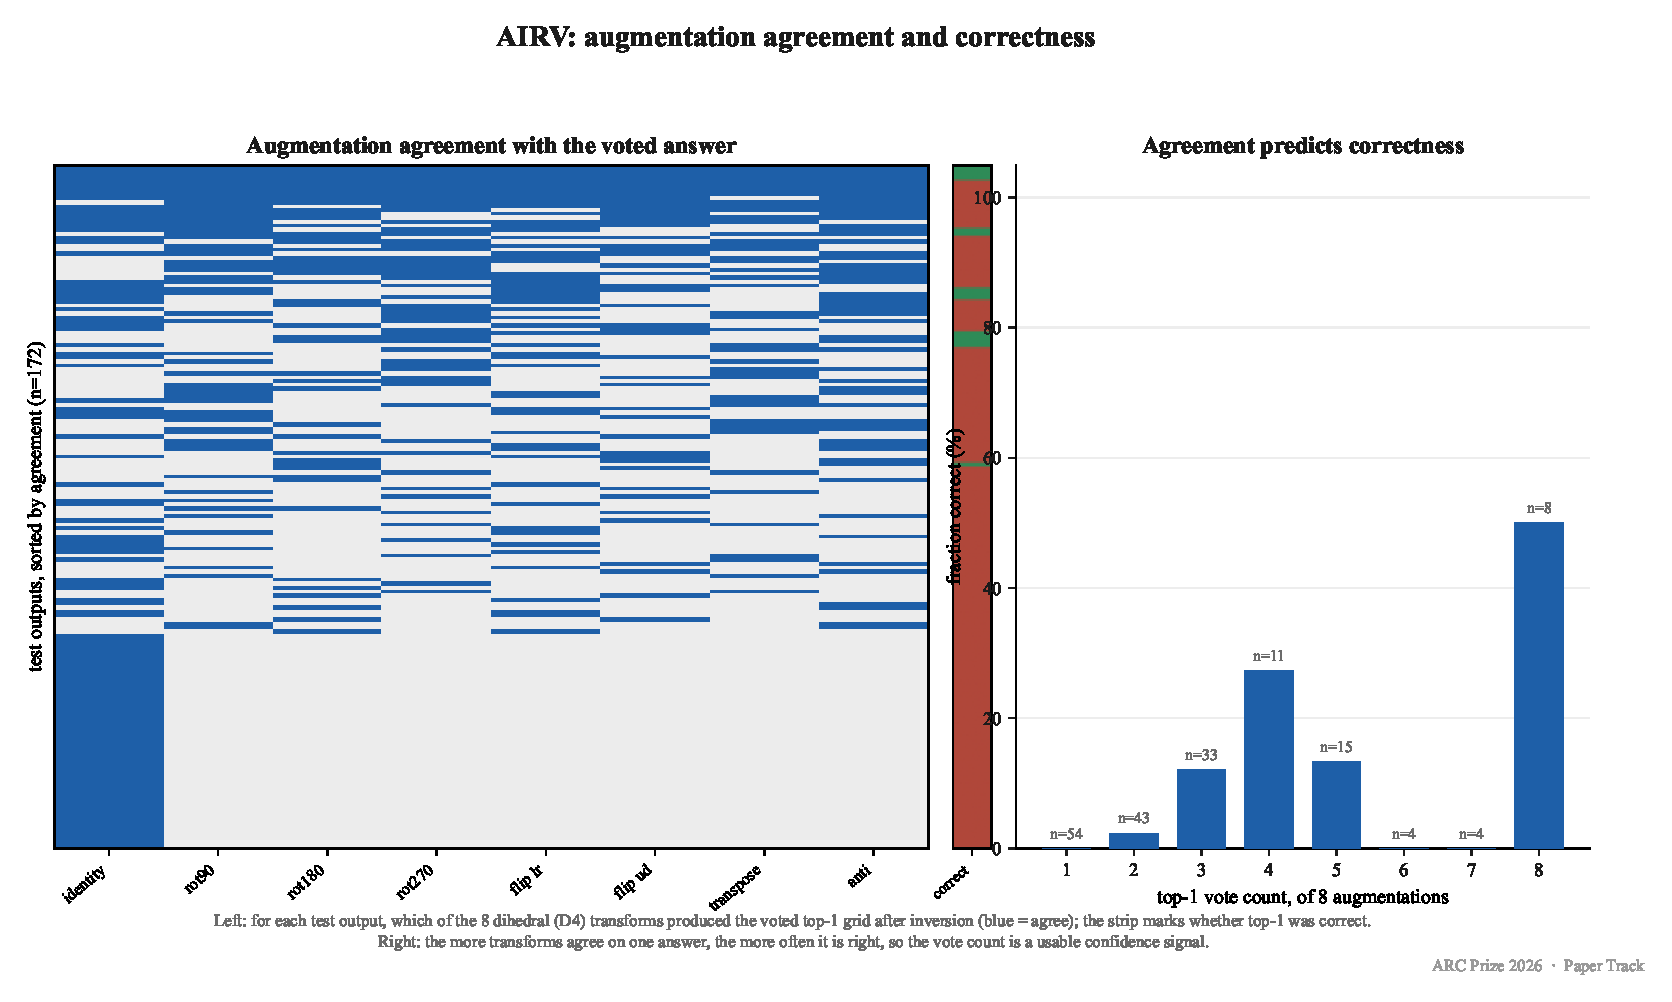
\includegraphics[width=\linewidth]{fig_airv_votes}
\end{minipage}
\caption{Left: which tasks TTT solves at each adapter scale, with most gains concentrated at scale
$1.25$. Right: AIRV vote agreement (Eq.~\eqref{eq:airv}) predicts correctness; full eight-way
consensus is right far more often than split votes.}
\label{fig:flip}
\label{fig:votes}
\end{figure}

\section{Discussion}
\label{sec:disc}

\subsection{Two lessons that generalize}
First, on a single GPU the inference engine is the dominant design choice; quantization and sampling
mattered far less than the $13\times$ we recovered by moving decode off the eager path. Second, the
real obstacle for TTT is the \emph{serving bridge}: training needs a gradient framework, fast
generation needs an optimized engine, and per-task TTT produces a fresh adapter the engine must
serve. We show this bridge is buildable on one card, and that once it exists the open question is not
plumbing but \emph{regularization}, because the small per-task training set overfits easily.

\subsection{Accuracy per GPU-hour}
We argue the right framing for compute-poor ARC work is \textbf{accuracy per GPU-hour}
(Figure~\ref{fig:cost}), and the map of walls reported here (the decode ceiling, the VRAM limit on
large-grid TTT, and the overfitting of naive adapters; Figure~\ref{fig:levers}) is a first step
toward it. The findings tell a practitioner with similar hardware exactly which problems to solve
first: fix the engine before touching anything else, budget VRAM by largest-train-pair length, and
regularize the per-task adapter rather than training it harder.

\begin{figure}[H]
\centering
\begin{minipage}{0.52\linewidth}\centering
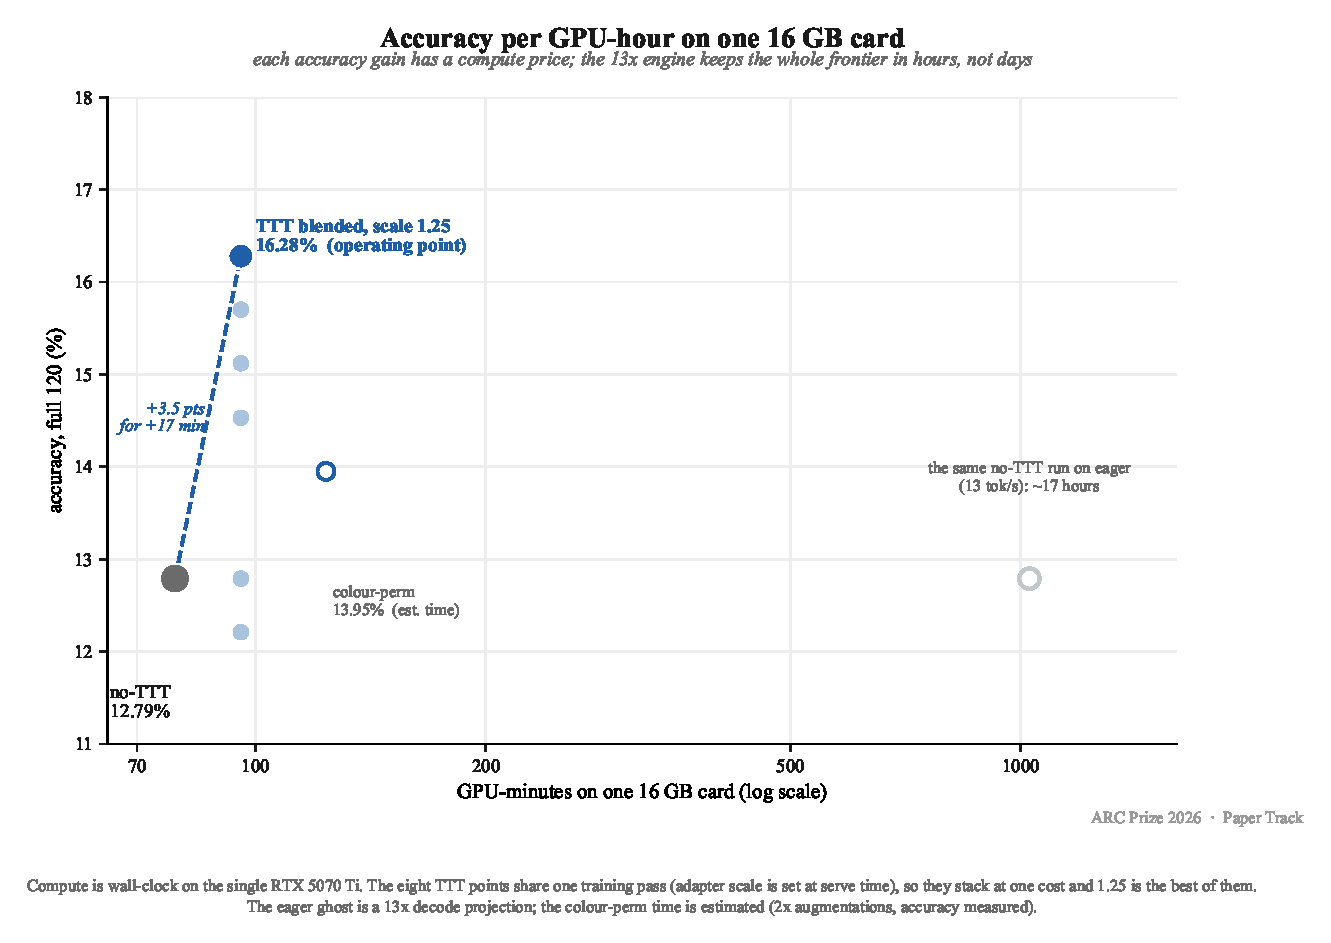
\includegraphics[width=\linewidth]{fig_cost_frontier}
\end{minipage}\hfill
\begin{minipage}{0.46\linewidth}\centering
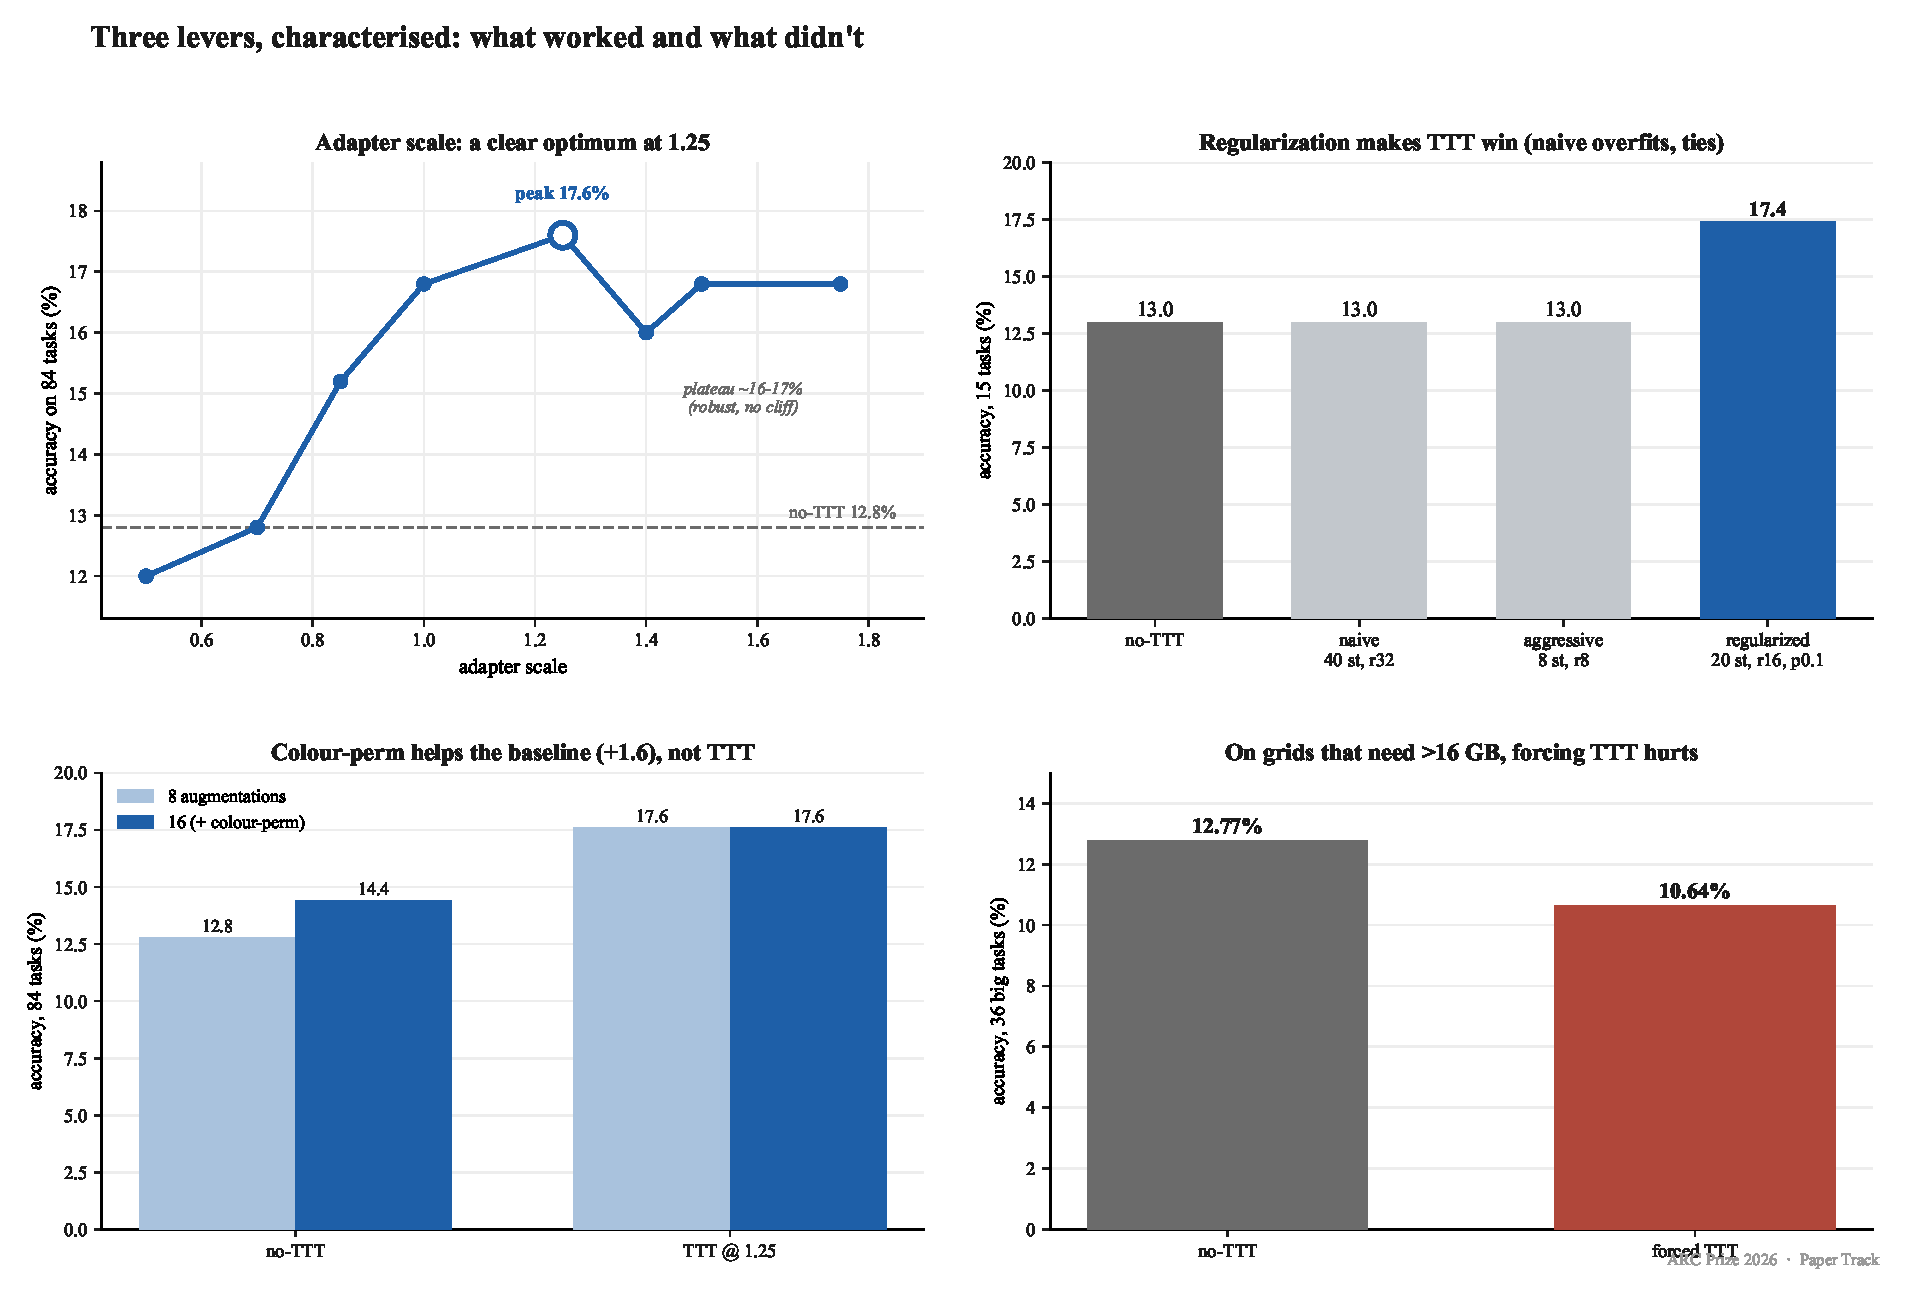
\includegraphics[width=\linewidth]{fig_levers}
\end{minipage}
\caption{Left: accuracy per GPU-hour on one card; the TTT blend at 16.28\% sits on the Pareto front
(compute is measured wall-clock, and any eager ``ghost'' points are $13\times$ projections, labelled
in the source). Right: what worked and what did not. The engine swap and regularized TTT helped,
while naive TTT, colour-perm stacking, and big-grid TTT did not.}
\label{fig:cost}
\label{fig:levers}
\end{figure}

\subsection{Limitations and ongoing work}
\label{sec:limits}
Our absolute accuracy is far below the 24.0\% cluster result, by design: one card and a fixed recipe.
The public-to-hidden gap is itself a finding: the no-TTT system scores 12.79\% on the public eval but
6.53\% on the hidden main-track set, a reminder that the public ARC-AGI-2 eval is more saturated than
the held-out sets, so a small single-GPU model carries less of its public accuracy across than a
cluster model would. A scored rerun can also lose the heaviest-grid tasks to server stalls, which our
next submission instruments (a per-task log) to separate empty answers from genuine misses.
The biggest known lever we still lack is verifier-guided selection and a refinement loop (generate,
check each candidate against the train pairs, then re-prompt on the discrepancy), which the 2025
analysis names as the central advance; our AIRV is a one-shot vote. We also probed whether a one-time continued LoRA fine-tune of the base on official ARC-AGI-2 training
data and RE-ARC~\cite{rearc} generations yields a better static model. It did not: the fine-tuned base
scores 11.63\% no-TTT against the stock base's 12.79\%, so we ship the stock base. The NVARC base is
already well-adapted to this grid format, and continued fine-tuning on this public data did not
transfer, a useful negative result for the compute-poor practitioner, more public data is not a free
lever once the base is task-tuned.

Building on that null result, we are extending the static fine-tune into an expert-iteration
self-training loop: the system solves the official training tasks with the current model, distils
the base on a curriculum of its own verified-correct solutions, then iterates. Exact-match grids
impose a sharp constraint: a verified-correct solution on a training task simply is its ground-truth
output, so a naive self-training corpus coincides with the data the continued fine-tune already used.
We confirm the trap empirically: an oracle any-match criterion saturates (the base reaches most
training tasks under some augmentation), so distilling on it would reproduce the null result above.
The lever that makes self-training a different experiment is the curriculum: we separate what the
base solves \emph{robustly} (the AIRV vote is correct) from what it merely \emph{reaches} (some
augmentation is correct), and distil only the gap, the near-miss tasks at the model's edge. The
keep/drop gate is unchanged (ship only if it beats the stock 12.79\% no-TTT and still stacks with
TTT), and the outcome is reported either way, a positive result as a better single-GPU operating
point or a second negative result on whether self-distillation can move ARC-AGI-2 once the base is
already task-tuned.

Finally, the significance of the TTT lift is directional
rather than conclusive (Appendix~\ref{app:results}); a full-eval paired run is the obvious next
measurement.

\section{Conclusion}
\label{sec:conclusion}
The 2025 winning recipe survives a single 16~GB consumer GPU, but only after the inference engine is
fixed: that one change is worth more than every other knob, and it is what makes per-task TTT
tractable through an adapter-serving bridge. The honest result is a 12.79\% no-TTT baseline and a
16.28\% regularized-TTT blend, with the gains bounded by adapter overfitting and a hard VRAM wall on
large grids. The full system is open source: the GGUF conversion recipe for the custom-vocabulary
model, the AIRV pipeline, the per-task TTT bridge and sweep harness, and a development log recording
every measurement and dead end behind these numbers.

\appendix

\section{Reproducibility}
\label{app:repro}

\textbf{Environment.} A single NVIDIA RTX~5070~Ti (16~GB, Blackwell, $\approx 896$~GB/s), native
Windows 11. Inference: a prebuilt llama.cpp CUDA~12.4 \texttt{llama-server}, run on Blackwell through
PTX JIT. Training: PyTorch with a LoRA via PEFT, bf16 base, gradient checkpointing. The two frameworks
are never co-resident in VRAM (Section~\ref{sec:ttt}).

\textbf{The two GGUF converter patches.} The NVARC model has a 16-token \emph{WordLevel} tokenizer,
which trips the stock converter twice. (1)~\emph{Unknown tokenizer hash:} the loader does not
recognize the tokenizer's hash and refuses to guess a pre-tokenizer; its pre-tokenizer is in fact the
\texttt{qwen2} regex, so we map the hash to \texttt{qwen2} explicitly. (2)~\emph{Empty merge list:} a
WordLevel tokenizer has no byte-pair merges, but the loader requires a non-empty list, so we add two
throwaway merges among the role tokens, which never fire on grid text. Both patches are in the
repository's conversion script and are applied automatically by the Kaggle prep notebook.

\textbf{Serving flags.} \texttt{llama-server} is launched with full GPU offload
(\texttt{-ngl~99}), a 16{,}384-token context, a single slot (\texttt{-np~1}), and the prompt cache
disabled (\texttt{--no-cache-prompt}); its own logs are redirected to a file so they never flood the
notebook. Decoding is greedy (temperature $0$) with \texttt{n\_predict} sized to the target grid.

\textbf{Hyperparameters.} AIRV uses the eight D4 augmentations and votes to two attempts. Per-task
TTT (regularized): rank 16 to 32, dropout 0.05 to 0.1, 8 to 20 steps, AdamW, a fresh random
augmentation per step, leave-one-out target, context capped at $\approx 1{,}600$ tokens, applied at
adapter scale $1.25$ at inference. Exact values per experiment are in the development log.

\section{Extended results}
\label{app:results}

\textbf{Per-scale accuracy (84 trainable tasks).} Table~\ref{tab:perscale} gives the full
adapter-scale sweep behind Figures~\ref{fig:results} and~\ref{fig:flip}. Accuracy rises to a peak at
scale~$1.25$ and then declines, the signature of an adapter applied too strongly.

\begin{table}[H]
\centering
\caption{No-TTT vs.\ TTT accuracy on the 84 trainable tasks as a function of adapter scale.}
\label{tab:perscale}
\begin{tabular}{lccccccccc}
\toprule
adapter scale & no-TTT & 0.50 & 0.70 & 0.85 & 1.00 & \textbf{1.25} & 1.40 & 1.50 & 1.75 \\
\midrule
accuracy (\%) & 12.8 & 12.0 & 12.8 & 15.2 & 16.8 & \textbf{17.6} & 16.0 & 16.8 & 16.8 \\
\bottomrule
\end{tabular}
\end{table}

\textbf{Paired significance.} On the 84 trainable tasks, TTT and no-TTT disagree on seven test
outputs: TTT is correct on six that no-TTT misses and incorrect on one that no-TTT gets. An exact
two-sided McNemar test on a $6/1$ split gives $p\approx0.13$, so the lift is not individually
significant; we report it as directional, corroborated by the configuration sweep ($+1$) and the
representativeness check (no-TTT scores 12.8\% on the subset versus 12.79\% on the full set).

\textbf{Colour permutation.} Adding a random colour permutation to the augmentation set lifts the
no-TTT baseline from 12.8\% to 14.4\% on the 84 tasks, but provides no further gain on top of the
per-task adapter, which has already learned the task's colour mapping, so the two do not stack.

\section{Engineering log: walls and dead ends}
\label{app:log}
We record the failures explicitly, because on this hardware they are most of the work.

\begin{itemize}[leftmargin=1.4em,itemsep=3pt]
\item \textbf{Eager decode is overhead-bound, and the usual fix is unavailable.} Hugging Face eager
decode runs at $\approx 13$ tok/s, about $10\%$ of the bandwidth roofline. \texttt{torch.compile}
would close the gap, but it needs Triton, which has no native-Windows backend. The resolution was to
change engines, not to optimize the eager path.
\item \textbf{The server prompt cache destabilizes unique-prompt workloads.} Enabled by default, it
reserves $\approx 680$~MiB per unique prompt; every ARC prompt is unique, so it never reuses and
instead destabilizes sustained generation. Disabling it and running a single supervised stream fixed
the stalls.
\item \textbf{4-bit QLoRA is broken on Blackwell + Windows.} bitsandbytes fails to load on this
platform, so the planned 4-bit continued fine-tune was infeasible. Because per-task TTT already runs
in bf16 inside 16~GB, we use a bf16 LoRA throughout and drop the 4-bit path entirely.
\item \textbf{PyTorch decode can turn quadratic after a training step.} Generation in the gradient
framework is not only slow but intermittently degrades after an optimizer step; this is precisely why
the serving bridge exists, since we never generate in PyTorch in the scored pipeline.
\item \textbf{The VRAM wall on large grids is real.} The largest-train-pair token length, not the
test grid size, is the binding constraint; tasks above the operational cutoff cannot train in 16~GB.
Forcing TTT onto them by truncation did not recover accuracy, so they are excluded and served no-TTT.
\item \textbf{Naive TTT ties the baseline.} The standard adapter configuration drives training loss
to $0.000$ and generalizes no better than no-TTT; only regularization (fewer steps, lower rank,
dropout) recovers a lift.
\end{itemize}

\section{Prompt and serialization format}
\label{app:format}
The model's 16-token vocabulary is given in Table~\ref{tab:vocab}. A grid is serialized row by row,
one token per cell (the token id equals the colour), rows separated by the newline token; prompts are
assembled at the id level as a ChatML few-shot sequence of train pairs followed by the test input,
ending at the \texttt{ASSISTANT} turn for the model to complete. Because the role and special tokens
have no textual spelling, the whole sequence is built from ids directly, never by tokenizing a
string, which is what guarantees parity between training and inference.

\begin{table}[H]
\centering
\caption{The 16-token grid vocabulary.}
\label{tab:vocab}
\begin{tabular}{ll}
\toprule
token ids & meaning \\
\midrule
0 to 9 & the ten ARC grid colours (id $=$ colour) \\
10   & newline / row separator \\
11   & \texttt{USER} role marker \\
12   & \texttt{ASSISTANT} role marker \\
13   & \texttt{PAD} \\
14   & \texttt{IM\_START} \\
15   & \texttt{IM\_END} \\
\bottomrule
\end{tabular}
\end{table}

\section{Data and model provenance}
\label{app:prov}
The base model is Qwen3-4B~\cite{qwen3} (Apache-2.0), supervised-fine-tuned on ARC grids by
NVARC~\cite{nvarc}; any derived weights we redistribute are released under Apache-2.0 with the
required \texttt{NOTICE}. Evaluation and training tasks are the official ARC-AGI-2 corpus~\cite{arcagi2}
(Apache-2.0); the in-progress fine-tune additionally uses RE-ARC~\cite{rearc} (MIT). Our own code and
weights are released under MIT-0. We never train on the evaluation tasks. Full license texts and
attribution are in the repository's \texttt{THIRD\_PARTY\_LICENSES.md} and \texttt{NOTICE}.

\medskip
\noindent\textbf{BibTeX.}
{\footnotesize
\begin{verbatim}
@article{chollet2019measure,
  title={On the Measure of Intelligence},
  author={Chollet, Francois}, journal={arXiv:1911.01547}, year={2019}}
@techreport{arcagi2,
  title={ARC-AGI-2 Technical Report},
  institution={ARC Prize Foundation}, year={2025}}
@techreport{arcprize2025,
  title={ARC Prize 2025: Technical Report},
  institution={ARC Prize Foundation}, note={arXiv:2601.10904}, year={2026}}
@misc{qwen3, title={Qwen3 Technical Report}, author={Qwen Team}, year={2025}}
@misc{nvarc2025,
  title={NVARC: ARC Prize 2025 (ARC-AGI-2) 1st-place solution},
  author={{NVIDIA Kaggle Grandmasters}}, year={2025}}
@article{hodel2024rearc,
  title={Addressing the Abstraction and Reasoning Corpus via
         Procedural Example Generation},
  author={Hodel, Michael}, journal={arXiv:2404.07353}, year={2024}}
\end{verbatim}
}

\begin{thebibliography}{9}
\bibitem{chollet} F.~Chollet. On the Measure of Intelligence. arXiv:1911.01547, 2019.
\bibitem{arcagi2} ARC Prize Foundation. ARC-AGI-2 Technical Report. 2025. \url{https://arcprize.org}.
\bibitem{arc2025} ARC Prize Foundation. ARC Prize 2025: Technical Report. arXiv:2601.10904, 2026.
\bibitem{nvarc} NVIDIA Kaggle Grandmasters (NVARC). ARC Prize 2025 (ARC-AGI-2) 1st-place solution. 2025.
\bibitem{qwen3} Qwen Team. Qwen3 Technical Report. 2025.
\bibitem{rearc} M.~Hodel. Addressing the Abstraction and Reasoning Corpus via Procedural Example
Generation. arXiv:2404.07353, 2024.
\end{thebibliography}

\end{document}
